\documentclass{beamer}
\usetheme{Madrid} % My favorite!
%\usetheme{Boadilla} % Pretty neat, soft color.
%\usetheme{default}
%\usetheme{Warsaw}
%\usetheme{Bergen} % This template has nagivation on the left
%\usetheme{Frankfurt} % Similar to the default 
%with an extra region at the top.
%\usecolortheme{seahorse} % Simple and clean template
%\usetheme{Darmstadt} % not so good
% Uncomment the following line if you want %
% page numbers and using Warsaw theme%
% \setbeamertemplate{footline}[page number]
%\setbeamercovered{transparent}
\setbeamercovered{invisible}
% To remove the navigation symbols from 
% the bottom of slides%
\setbeamertemplate{navigation symbols}{} 
%
\usepackage{graphicx}
%\usepackage{bm}         % For typesetting bold math (not \mathbold)
%\logo{\includegraphics[height=0.6cm]{yourlogo.eps}}
%
\title[ImageNet]{ImageNet Classification}
\author{Sunpreet Arora \& Josh Klontz}
\date{\today}
% \today will show current date. 
% Alternatively, you can specify a date.
%
\begin{document}
%
\begin{frame}
\titlepage
\end{frame}
%
\begin{frame}
\frametitle{Motivation}
\begin{block}
{Why Beamer?}
Does anybody need an introduction to Beamer? I don't think so.
\end{block}
\end{frame}
%
\begin{frame}
\frametitle{Multi-Scale Dense Feature Extraction}
\begin{columns}
\begin{column}{.5\textwidth}
\begin{figure}
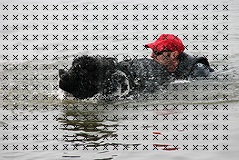
\includegraphics[height=1.5in]{dog_intdet}
\caption{Dense sampling at 3 scales}
\end{figure}
\end{column}
\pause
\begin{column}{.5\textwidth}
\begin{figure}
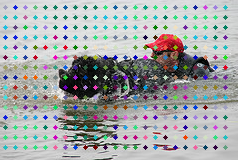
\includegraphics[height=1.5in]{dog_quantized}
\caption{Bag of words}
\end{figure}
\end{column}
\end{columns}
\end{frame}
%
\begin{frame}[fragile] % Notice the [fragile] option %
\frametitle{Verbatim}
\begin{example}[Putting Verbatim]
\begin{verbatim}
\begin{frame}
\frametitle{Outline}
\begin{block}
{Why Beamer?}
Does anybody need an introduction to Beamer?
I don't think so.
\end{block}
% Extra carriage return causes problem with verbatim %
\end{frame}\end{verbatim} 
\end{example}
\end{frame}
 
\begin{frame}[fragile]  % notice the fragile option, since the body
			% contains a verbatim command
Example of the \verb|\cite| command to give a reference is below:
Example of citation using \cite{key1} follows on.
\end{frame}
 
\begin{frame}
\frametitle{References}
\footnotesize{
\begin{thebibliography}{99}
 \bibitem[Label1, 2010]{key1} Author's name (1987)
 \newblock Title of the paper.
 \newblock \emph{Journal Name} 55(4), 765 -- 799.
\end{thebibliography}
}
\end{frame}
 
\begin{frame}
\centerline{The End}
\end{frame}
% End of slides
\end{document} 